\documentclass{article}
\usepackage{amsmath}
\usepackage{graphicx}
\begin{document}
\author{Ana Bhattacharjee}
\title{Quiz 2: Question 34}
\date{\today}
\maketitle{}

\begin{center}
The question says that the shape of the garden will be a rectangle. A plot of the rectangular garden is shown below.
\begin{figure}[!htbp]
  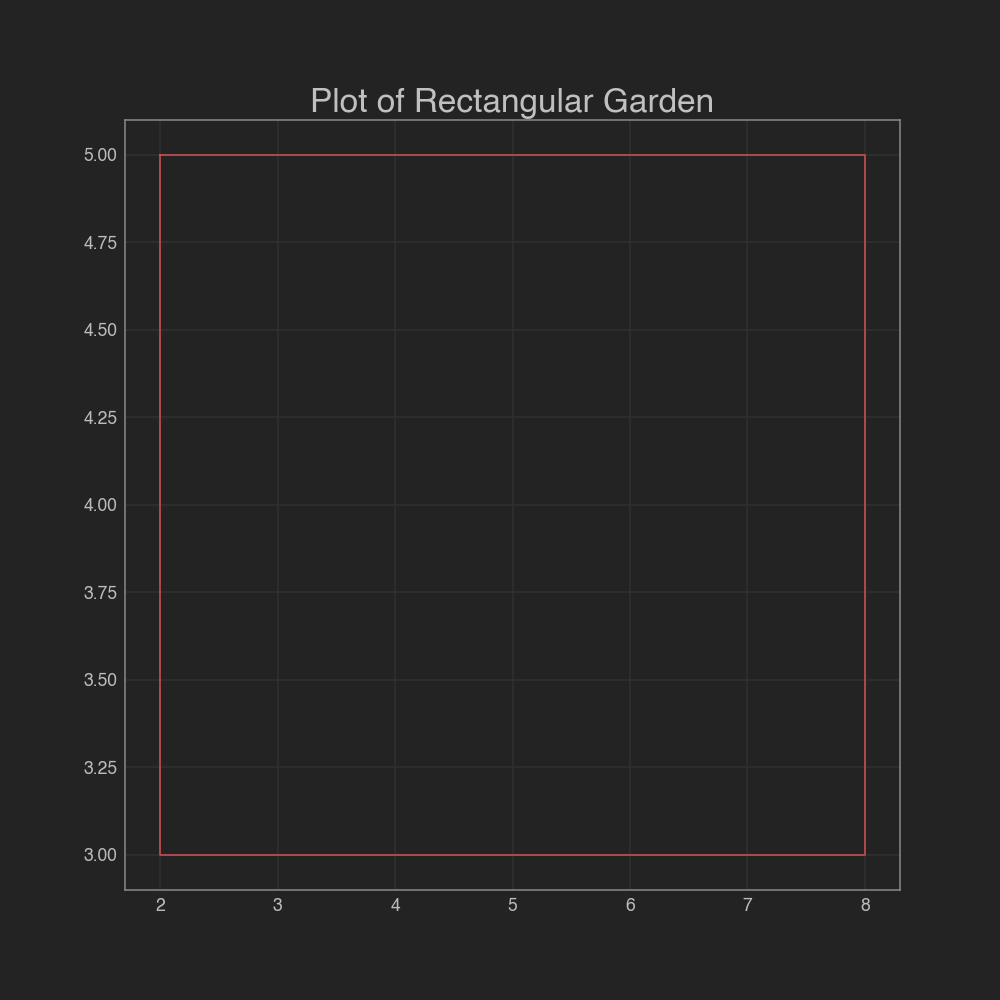
\includegraphics[width=0.9\columnwidth]{../../../../../../math/Anna/geometry/coordinate_geometry/quiz2/q34/rectangular_garden}
  \caption{Rectangular Garden}
\end{figure}
\par
As seen from above, one can easily see that the length of the garden is 6 units and the width of the garden is 2 units. Calculation of the rectangular garden's area is shown below.
\begin{align}
  A = l * w \\
  A = 6 * 2 = 12 \vspace{1cm} \text{units}^2
\end{align}
Now that the area has been calculated, we must divide the garden's area by the area that each bag of mulch covers.
\begin{align}
  n_{\text{bags}} = \frac{A_1}{A_2} \rightarrow \frac{12}{6} = 2 \vspace{1cm} \text{bags} \\
\end{align}
Finally, we multiply the number of bags by the cost of each bag.
\begin{align}
  \text{total} = n_{\text{bags}} * \text{cost} \\
  \text{total} = 2 * 5.25 \\
  \text{total} = \$ 10.50
\end{align}
\end{center}


\end{document}
